% !TeX program = pdflatex
\documentclass[conference]{IEEEtran}
\IEEEoverridecommandlockouts
% The preceding line is only needed to identify funding in the first footnote. If that is unneeded, please comment it out.
\usepackage{cite}
\usepackage{amsmath,amssymb,amsfonts}
\usepackage{algorithmic}
\usepackage{graphicx}
\usepackage{textcomp}
\usepackage{xcolor}
\usepackage{tikz}
\usepackage{pgfplots}
\pgfplotsset{compat=1.16}
\usepackage{booktabs}
\usepackage{siunitx}
\usepackage{hyperref}
\usepackage{fancyhdr}
\hypersetup{
    colorlinks=true,
    linkcolor=blue,
    filecolor=magenta,      
    urlcolor=cyan,
    citecolor=blue,
}

% Set up fancy headers
\pagestyle{fancy}
\fancyhf{}
\setlength{\headheight}{25.81677pt}
\addtolength{\topmargin}{-13.81677pt}
\fancyhead[C]{}
\fancyfoot[C]{\includegraphics[width=0.5cm]{feutech_seal.png}}
\renewcommand{\headrulewidth}{0pt}

\begin{document}

\title{\includegraphics[width=0.6\textwidth]{headlogocut.png}\\[1cm]Usability Analysis of Amazon's E-Commerce Platform: A Mixed-Methods Study}

\author{\IEEEauthorblockN{Artainian Abulencia, Vinz Angelo De Guzman, Gio Carlo Panopio, Angelo Manalo}
\IEEEauthorblockA{Human-Computer Interaction\\
FEU Institute of Technology\\
Manila, Philippines\\
\{202411201, 202411330, 202411316, 202410769\}@fit.edu.ph}}

\maketitle

\begin{abstract}
This study assesses the usability of Amazon's e-commerce platform through a mixed-methods approach, integrating survey data from 13 participants and usability testing results. Findings indicate that Amazon excels in layout intuitiveness (84.6\% positive ratings), recommendation effectiveness (84.6\%), and transaction security perceptions (84.6\%), yet struggles with interface clutter, navigation challenges, and delivery concerns. Quantitative metrics, such as an average satisfaction score of 2.08/3 and a Net Promoter Score (NPS) of 15.5, suggest moderate user satisfaction with potential for enhancement. The System Usability Scale (SUS) score of 74/100 fell below the target of 80/100, indicating room for improvement. Recommendations include reducing visual clutter, improving search functionality, and enhancing delivery communication to elevate the overall user experience.
\end{abstract}

\begin{IEEEkeywords}
e-commerce, usability testing, user experience, human-computer interaction, Amazon
\end{IEEEkeywords}

\section{Introduction}
Usability is a cornerstone of successful e-commerce platforms, directly impacting user satisfaction, retention, and business performance. As a leader in online retail, Amazon's website serves millions daily, making its usability a critical factor in maintaining competitive advantage. This study investigates Amazon's user experience by analyzing survey data and usability testing results, focusing on interface design, navigation, search functionality, checkout processes, and delivery experiences.

The research originated from an HCI course project outlined in the project guidelines, where we were tasked with analyzing provided survey data and a usability study report on Amazon's website, identifying usability issues, and proposing improvements based on HCI principles. This paper consolidates those efforts, offering a detailed evaluation and actionable recommendations to enhance Amazon's usability for its diverse user base.

\section{Methodology}
A mixed-methods approach was employed to comprehensively evaluate Amazon's usability, combining quantitative survey data and qualitative usability testing insights.

\subsection{Survey Design}
The survey collected responses from 13 participants—primarily students aged 18-22—on various usability aspects:
\begin{itemize}
    \item \textbf{Quantitative Metrics:} Ratings for layout intuitiveness, navigation ease, overall satisfaction (1-3 scale), recommendation likelihood (1-4 scale), and security perceptions.
    \item \textbf{Qualitative Feedback:} Open-ended comments on challenges and improvement suggestions.
\end{itemize}

\subsection{Usability Testing}
Usability testing assessed user interactions with Amazon's desktop and mobile web interfaces through tasks such as:
\begin{itemize}
    \item Locating and purchasing a product
    \item Navigating to deals and managing the cart
    \item Completing checkout
    \item Comparing products
    \item Updating account preferences
\end{itemize}

Key metrics included task completion rates, time on task, error rates, and satisfaction scores, with a target System Usability Scale (SUS) score of 80/100 as a benchmark for good usability.

\section{Findings}
The analysis revealed Amazon's usability strengths and areas needing improvement, supported by both survey data and usability testing outcomes.

\subsection{User Interface and Navigation}
\begin{itemize}
    \item \textbf{Strengths:} 84.6\% of participants rated the layout as "Intuitive" or "Very Intuitive," and 84.6\% found product location "Easy" or "Very Easy." In usability testing, the task of finding and purchasing a specific product had an 85\% success rate, with an average completion time of 3.2 minutes.
    \item \textbf{Challenges:} 38.5\% reported interface clutter and excessive advertisements as significant issues, with comments like "UI is very cluttered." Usability testing showed that 25\% of users struggled with filtering options during product search. Navigation difficulties, such as accessing the cart, were also noted.
\end{itemize}

\begin{table}[!htbp]
\caption{User Ratings for Interface and Navigation}
\label{table:ui_navigation}
\centering
\begin{tabular}{@{}lccc@{}}
\toprule
\textbf{Aspect} & \textbf{Very Positive} & \textbf{Positive} & \textbf{Negative} \\
\midrule
Layout Intuitiveness & Very Intuitive: 15.4\% & Intuitive: 69.2\% & Unintuitive: 15.4\% \\
Product Location & Very Easy: 15.4\% & Easy: 69.2\% & Difficult: 15.4\% \\
\bottomrule
\end{tabular}
\end{table}

\subsection{Product Search and Information Architecture}
\begin{itemize}
    \item \textbf{Strengths:} 84.6\% rated recommendations and customer reviews as "Effective" or "Very Effective."
    \item \textbf{Challenges:} 7.7\% struggled to find specific items, with one participant suggesting "better indicators for sold-out products." Usability testing revealed that 35\% of users relied on category navigation rather than search, indicating potential search inefficiencies.
\end{itemize}

\subsection{Transaction Security and Checkout}
\begin{itemize}
    \item \textbf{Strengths:} 84.6\% felt "Secure" or "Very Secure" during transactions.
    \item \textbf{Challenges:} 15.4\% reported feeling "Insecure," posing a risk to trust and conversion rates. During usability testing, 80\% of participants completed the checkout process without assistance, but 40\% were confused by multiple delivery options.
\end{itemize}

\subsection{Delivery Experience}
\begin{itemize}
    \item \textbf{Strengths:} 84.6\% were "Satisfied" or "Very Satisfied" with delivery speed.
    \item \textbf{Challenges:} 23.1\% highlighted delivery delays, with one noting "late deliveries" as a recurring issue.
\end{itemize}

\subsection{Overall Satisfaction and Loyalty}
\begin{itemize}
    \item \textbf{Satisfaction:} Average score of 2.08/3, indicating moderate satisfaction.
    \item \textbf{Net Promoter Score (NPS):} Calculated at 15.5 (Promoters: 38.5\%, Detractors: 23.1\%), suggesting positive but improvable user advocacy.
    \item \textbf{System Usability Scale (SUS):} The overall SUS score was 74/100, falling short of the target of 80/100.
\end{itemize}

\begin{table}[!htbp]
\caption{Satisfaction and Recommendation Distribution}
\label{table:satisfaction}
\centering
\begin{tabular}{@{}lcccc@{}}
\toprule
\textbf{Metric} & \textbf{1 (Best)} & \textbf{2} & \textbf{3} & \textbf{4 (Worst)} \\
\midrule
Satisfaction & 23.1\% & 46.1\% & 30.8\% & - \\
Recommend Likelihood & 38.5\% & 38.5\% & 7.7\% & 15.4\% \\
\bottomrule
\end{tabular}
\end{table}

\begin{figure}[!htbp]
\centering
\begin{tikzpicture}
\begin{axis}[
    ybar,
    bar width=20pt,
    width=0.9\linewidth,
    height=5cm,
    legend style={at={(0.5,1.05)}, anchor=south, legend columns=3},
    ylabel={Percentage (\%)},
    symbolic x coords={Layout, Navigation, Security, Recommendations, Delivery},
    xtick=data,
    nodes near coords,
    ymin=0, ymax=100,
    x tick label style={rotate=45, anchor=east},
    title={Key Usability Metrics - Positive Ratings},
]
\addplot coordinates {(Layout, 84.6) (Navigation, 84.6) (Security, 84.6) (Recommendations, 84.6) (Delivery, 84.6)};
\end{axis}
\end{tikzpicture}
\caption{Positive user ratings across key usability dimensions}
\label{fig:positive_ratings}
\end{figure}

\begin{figure}[!htbp]
\centering
\begin{tikzpicture}
\begin{axis}[
    width=0.9\linewidth,
    height=5cm,
    xlabel={Metric},
    ylabel={Score},
    symbolic x coords={SUS (target), SUS (actual), Satisfaction, NPS},
    xtick=data,
    ymin=0, ymax=100,
    nodes near coords,
    title={Overall Performance Metrics},
    x tick label style={rotate=45, anchor=east}
]
\addplot[ybar, fill=blue!30] coordinates {
    (SUS (target), 80)
    (SUS (actual), 74)
    (Satisfaction, 69.3)
    (NPS, 15.5)
};
\end{axis}
\end{tikzpicture}
\caption{Comparison of overall performance metrics}
\label{fig:performance_metrics}
\end{figure}

\section{Discussion}
The findings highlight usability issues that violate key HCI principles, providing a framework for understanding their impact on user experience.

\subsection{Interface Clutter and Advertisements}
\begin{itemize}
    \item \textbf{Issue:} 38.5\% of participants found the interface cluttered due to ads.
    \item \textbf{HCI Principle:} Violates Nielsen's \textit{Aesthetic and Minimalist Design} heuristic, overwhelming users with non-essential content.
    \item \textbf{Severity:} High (P1) – frequent complaints disrupt task efficiency.
\end{itemize}

\subsection{Navigation and Search Functionality}
\begin{itemize}
    \item \textbf{Issue:} Challenges in locating products and accessing the cart.
    \item \textbf{HCI Principle:} Contravenes \textit{Recognition Rather Than Recall}, requiring users to remember pathways rather than recognize them.
    \item \textbf{Severity:} Medium (P2) – impacts efficiency but mitigated by familiarity.
\end{itemize}

\subsection{Security Perceptions}
\begin{itemize}
    \item \textbf{Issue:} 15.4\% felt insecure during transactions.
    \item \textbf{HCI Principle:} Undermines \textit{Trust and Credibility}, essential for e-commerce platforms.
    \item \textbf{Severity:} Critical (P0) – low frequency but high impact on user trust.
\end{itemize}

\subsection{Delivery Concerns}
\begin{itemize}
    \item \textbf{Issue:} 23.1\% reported delivery delays as a major issue.
    \item \textbf{HCI Principle:} Affects \textit{Visibility of System Status}, leaving users uncertain about order progress.
    \item \textbf{Severity:} High (P1) – influences post-purchase satisfaction and loyalty.
\end{itemize}

\begin{figure}[!htbp]
\centering
\begin{tikzpicture}
\begin{axis}[
    ybar,
    bar width=15pt,
    width=0.9\linewidth,
    height=5cm,
    legend style={at={(0.5,1.05)}, anchor=south, legend columns=2},
    ylabel={Percentage (\%)},
    symbolic x coords={Interface Clutter, Navigation Issues, Security Concerns, Delivery Problems},
    xtick=data,
    nodes near coords,
    ymin=0, ymax=50,
    x tick label style={rotate=45, anchor=east},
    title={Reported Usability Issues},
]
\addplot coordinates {(Interface Clutter, 38.5) (Navigation Issues, 15.4) (Security Concerns, 15.4) (Delivery Problems, 23.1)};
\end{axis}
\end{tikzpicture}
\caption{Frequency of reported usability issues}
\label{fig:usability_issues}
\end{figure}

\section{Recommendations}
The following recommendations address identified issues, prioritized by severity and supported by measurable outcomes. These are informed by HCI principles and best practices for e-commerce usability.

\subsection{High-Priority Interface Improvements}
\begin{enumerate}
    \item \textbf{Reduce Visual Clutter}: Increase white space and use progressive disclosure for secondary content.
    \begin{itemize}
        \item \textit{Metric:} Reduce average product search time by 20\%.
    \end{itemize}
    \item \textbf{Integrate Ads Seamlessly}: Allow users to customize ad visibility.
    \begin{itemize}
        \item \textit{Metric:} Decrease task abandonment rate by 15\%.
    \end{itemize}
    \item \textbf{Enhance Navigation}: Improve cart visibility and simplify menu structures.
    \begin{itemize}
        \item \textit{Metric:} Increase cart access success rate to 95\%.
    \end{itemize}
\end{enumerate}

\subsection{Product Information Enhancements}
\begin{enumerate}
    \item \textbf{Real-Time Stock Indicators}: Clearly mark product availability.
    \begin{itemize}
        \item \textit{Metric:} Reduce searches for unavailable items by 25\%.
    \end{itemize}
    \item \textbf{Advanced Search Features}: Add faceted search and autocomplete options.
    \begin{itemize}
        \item \textit{Metric:} Increase first-try search success rate to 90\%.
    \end{itemize}
    \item \textbf{User Guidance}: Offer optional tutorials for new users.
    \begin{itemize}
        \item \textit{Metric:} Improve novice satisfaction by 10\%.
    \end{itemize}
\end{enumerate}

\subsection{Security and Trust Enhancements}
\begin{enumerate}
    \item \textbf{Reinforce Security Cues}: Display certifications during checkout.
    \begin{itemize}
        \item \textit{Metric:} Reduce "Insecure" ratings to below 5\%.
    \end{itemize}
    \item \textbf{Streamline Authentication}: Simplify sign-in with visible security indicators.
    \begin{itemize}
        \item \textit{Metric:} Decrease sign-in time by 15\%.
    \end{itemize}
    \item \textbf{Seller Oversight}: Enhance scam detection mechanisms.
    \begin{itemize}
        \item \textit{Metric:} Reduce scam reports by 30\%.
    \end{itemize}
\end{enumerate}

\subsection{Delivery and Fulfillment Improvements}
\begin{enumerate}
    \item \textbf{Accurate Delivery Estimates}: Leverage data for realistic timelines.
    \begin{itemize}
        \item \textit{Metric:} Achieve 95\% on-time delivery.
    \end{itemize}
    \item \textbf{Improved Tracking}: Provide frequent status updates.
    \begin{itemize}
        \item \textit{Metric:} Increase delivery satisfaction to 90\%.
    \end{itemize}
    \item \textbf{Flexible Options}: Allow customizable delivery preferences.
    \begin{itemize}
        \item \textit{Metric:} Boost preference usage by 20\%.
    \end{itemize}
\end{enumerate}

\subsection{Validation Through A/B Testing}
Implement A/B testing using tools like Google Analytics Content Experiments to validate design changes and measure improvements in user satisfaction and task completion rates.

\begin{figure}[!htbp]
\centering
\begin{tikzpicture}
\begin{axis}[
    width=0.9\linewidth,
    height=7cm,
    title={Prioritization Matrix of Recommendations},
    xlabel={Implementation Difficulty},
    ylabel={User Impact},
    xmin=0, xmax=10,
    ymin=0, ymax=10,
    grid=both,
    minor grid style={gray!25},
    major grid style={gray!25},
    scatter/classes={
        a={mark=square*,blue},
        b={mark=triangle*,red},
        c={mark=o,green!50!black}
    },
    legend style={at={(0.5,-0.20)}, anchor=north, font=\small, legend columns=3},
    legend entries={\textbf{High Priority}, \textbf{Medium Priority}, \textbf{Low Priority}}
]
\addplot[scatter,only marks,
    scatter src=explicit symbolic,
    mark size=4pt] 
    table[meta=class] {
        x y class
        8 9 a
        6 7 a
        7 6 a
        9 8 b
        5 9 b
        7 8 b
        3 4 c
        4 5 c
        2 6 c
    };
\end{axis}
\end{tikzpicture}
\caption{Prioritization of key recommendations by impact and difficulty. High Priority: Reduce Clutter (8,9). Medium Priority: Security Cues (9,8), Delivery Updates (7,8).}
\label{fig:priority_matrix}
\end{figure}

\section{Conclusion}
Amazon's platform demonstrates significant usability strengths in layout intuitiveness, recommendations, and security, yet faces critical challenges with interface clutter (P1), delivery delays (P1), and security perceptions (P0). Implementing the proposed recommendations—such as decluttering the interface, enhancing search capabilities, and improving delivery transparency—can elevate user satisfaction and loyalty, ultimately benefiting business outcomes. Future research should expand participant diversity and incorporate longitudinal metrics to further validate these insights.

\begin{thebibliography}{00}
\bibitem{survey} ``Survey Data,'' Retrieved from https://ppl-ai-file-upload.s3.amazonaws.com/web/direct-files/41956962/937397dc-a49f-41a7-88bc-6ce7bac1ee44/survey.csv
\bibitem{usability} ``Usability Study Report,'' Retrieved from https://ppl-ai-file-upload.s3.amazonaws.com/web/direct-files/41956962/c189a817-1061-4059-a42e-40d0ad4c4de9/docs.md
\bibitem{project} ``Project Guidelines,'' Retrieved from https://ppl-ai-file-upload.s3.amazonaws.com/web/direct-files/41956962/e5b2b846-d9a3-49c4-97e6-c1559812c8cb/guide.md
\bibitem{nielsen} J. Nielsen, ``10 Usability Heuristics for User Interface Design,'' Nielsen Norman Group, 1994. [Online]. Available: https://www.nngroup.com/articles/ten-usability-heuristics/
\bibitem{crazyegg} Crazy Egg, ``5 Fundamental Guidelines for Ecommerce Usability Design,'' [Online]. Available: https://www.crazyegg.com/blog/ecommerce-usability-design/
\bibitem{googleanalytics} Google, ``Content Experiments,'' Google Analytics Help. [Online]. Available: https://support.google.com/analytics/answer/1745147?hl=en
\end{thebibliography}

\end{document}